\documentclass[a4paper, 11pt]{article}
\usepackage{graphicx}
\usepackage{amsmath}
\usepackage{float}
\usepackage{hyperref}
\usepackage[inner=1in, top=1in, bottom=1in]{geometry}
\usepackage{amsfonts}
\usepackage{color,soul}
\usepackage{framed}
\DeclareMathOperator{\Cor}{Cor}
\DeclareMathOperator{\Cov}{Cov}
\DeclareMathOperator{\STD}{STD}
\DeclareMathOperator{\Var}{Var}
\DeclareMathOperator{\E}{E}
\DeclareMathOperator{\Tr}{Tr}
\DeclareMathOperator{\diag}{diag}
\DeclareMathOperator{\x}{\boldsymbol{x}}
\DeclareMathOperator{\X}{\boldsymbol{X}}
\DeclareMathOperator{\y}{\boldsymbol{y}}
\DeclareMathOperator{\z}{\boldsymbol{z}}
\DeclareMathOperator{\f}{\boldsymbol{f}}
\DeclareMathOperator{\bmu}{\boldsymbol{\mu}}
\DeclareMathOperator{\bSigma}{\boldsymbol{\Sigma}}

\begin{document}

\title{A Tutorial on Sparse Variational Gaussian Processes}
\author{P.L.Green\\
Institute for Risk and Uncertainty\\
School of Engineering\\
University of Liverpool\\
Liverpool, L69 7ZF\\
United Kingdom\\
\\
\href{mailto:p.l.green@liverpool.ac.uk}{p.l.green@liverpool.ac.uk} \\
\url{https://www.liverpool.ac.uk/engineering/staff/peter-green/}
}
\maketitle

%%%%%%%%%%%%%%%%%%%%%%%%%%%%%%%%%%%%%%%%%%%%%%%%%%%%%%%%%%%%%%%%%%%%%%%%%%
\section*{Acknowledgments}
Thank you to Ryan Jackson (University of Liverpool, UK) and Kaikai Zhao (Indiana University, Bloomington, USA) for their feedback!

%%%%%%%%%%%%%%%%%%%%%%%%%%%%%%%%%%%%%%%%%%%%%%%%%%%%%%%%%%%%%%%%%%%%%%%%%%
\section{Introduction}
This document is supposed to provide a tutorial-style introduction to Sparse Variational Gaussian Processes which are typically able to analyse larger data sets than standard Gaussian Processes. As with our other tutorials, the current document is accompanied by some example Python code. The code is heavily commented and is designed to help those new to the topic. It is recommended that this tutorial should only be studied once a basic understanding of standard Gaussian Processes has been established. We offer such a tutorial here: \url{https://github.com/plgreenLIRU/Gaussian-Process-regression-tutorial}. \\

%%%%%%%%%%%%%%%%%%%%%%%%%%%%%%%%%%%%%%%%%%%%%%%%%%%%%%%%%%%%%%%%%%%%%%%%%%
\section{Tutorial Structure}
The tutorial is structured as follows. A general overview of the approach behind Sparse Variational Gaussian Processes (herein simply referred to as `Sparse GPs') as well as a summary of key results is given in Section \ref{sec:overview}. Example code is then described immediately afterwards, in Section \ref{sec:code}. At this point the reader may wish to stop, however, for those wanting more information, more detailed derivations are then given in Section \ref{sec:details} before a summary of some interesting references is given in Section \ref{sec:refs}.\\

%%%%%%%%%%%%%%%%%%%%%%%%%%%%%%%%%%%%%%%%%%%%%%%%%%%%%%%%%%%%%%%%%%%%%%%%%%
\section{Overview}\label{sec:overview}
In this tutorial, we specifically consider regression problems where we define $\y = (y_1,...,y_N)^T$ as noisy observations of a function, $f$, at inputs $\X = \{\x_1,...,\x_N\}$, such that our full set of training data is $(\x_1,y_1),...,(\x_N,y_N)$. We assume that our observations are made according to the noise model

\begin{equation}
	y_i = f(\x_i) + \epsilon, \qquad \epsilon \sim \mathcal{N}(\epsilon;0,\sigma^2)	
\end{equation}
Using the notation $f_i \equiv f(\x_i)$, the vector of true function values is written as $\f = (f_1,...,f_N)^T$. If $N$ is large, computational cost often prevents us from using `standard' GPs. With the Variational Sparse GP described in \cite{Titsias2009} and \cite{Titsias2009a}, we train our GP on a smaller set of data, consisting of observations at the set of inputs $\X_m = \{ \x_{m,1},...,\x_{m,M} \}$ (where, for this tutorial, we will assume that $\X_m$ is a subset of $\X$). The aim is to make the Sparse GP `look like' a standard GP that had been trained on the full set of training data as closely as possible. This approach therefore assumes that there is some redundancy in our data - it builds on the idea that we only really need a small subset of `important' points to get a reasonable estimate of the true function, $f$.\\

Stated briefly, we proceed in 3 key steps. These are described in the boxes below: 

\begin{framed}
\subsection*{Step 1: Define the optimum inducing points.} 
In the following, we define the set of inputs $\X_m$ as `inducing points'. As a first step, we have to define what we mean by the \emph{optimum} set of inducing points - in other words, we ask the question: what do we use to help us choose the `best' $\X_m$? \\

Say $\f_m$ is the vector of true function values at the points in $\X_m$ (such that $f_{m,i} \equiv f(\x_{m,i})$). We begin by stating that the optimum choice of $\X_m$ would lead to $\f_m$ such that

\begin{equation}
	p(\y|\f_m) = p(\y|\f,\f_m)
\end{equation}
(where dependence on $\X$ and $\X_m$ isn't written for notational simplicity). Essentially, if we pick the best possible $\f_m$, then knowing $\f$ wouldn't change the probability of witnessing the observations $\y$. It turns out that enforcing this condition implies the following factorisation of our posterior probability distribution over $\f$ and $\f_m$:

\begin{equation}
	p(\f,\f_m|\y) = p(\f_m|\y)p(\f|\f_m)
	\label{SparseGP_PosteriorFactorisation}
\end{equation}
From this we conclude that a good choice of $\X_m$ is one that leads to equation (\ref{SparseGP_PosteriorFactorisation}) being true. 

\end{framed}


\begin{framed}
\subsection*{Step 2: Variational Bayes framework}
Briefly stated, variational Bayesian approaches involve the construction of a \emph{variational distribution}, $q$, that closely approximates some distribution of interest. A good choice of variational distribution is usually defined as that which minimises the \emph{KL divergence} between $q$ and the distribution of interest (see \cite{mackay2003information}\cite{Bishop2013} for more information). \\

In our case, we choose to approximate the posterior with the PDF, $p(\f,\f_m|\y)$, with 

\begin{equation}
	q(\f,\f_m) = \phi(\f_m)p(\f|\f_m)
\end{equation}
where $\phi(\f_m)$ is a PDF that is currently unknown. We hypothesise that, if we pick the optimum $\f_m$, then the posterior will factorise as shown in equation (\ref{SparseGP_PosteriorFactorisation}) and it would then be possible to find the distribution, $\phi(\f_m)$, that sets the KL divergence between $p(\f,\f_m|\y)$ and $q(\f,\f_m)$ equal to zero. Conveniently, we know that minimising the KL divergence is equivalent to maximising a lower bound on the log marginal likelihood, which we denote as $L$ (again, see \cite{mackay2003information}\cite{Bishop2013} for more details).
\end{framed}

\begin{framed}
\subsection*{Step 3: Maximise a lower bound}
Rather than maximising $L$ directly it turns out that, by instead maximising a lower bound on $L$, we can still select some `good' inducing points while avoiding having to find the variational distribution $\phi(\f_m)$. This lower bound on $L$ is denoted $L_{lb}$, and is given by

\begin{equation}
L_{lb} = \log\left[ \mathcal{N}(\y; \boldsymbol{0}, \boldsymbol{I}_n\sigma^2 + \boldsymbol{K}_{nm}\boldsymbol{K}_{mm}^{-1}\boldsymbol{K}_{mn})\right] -\frac{1}{2\sigma^2} \Tr\left(  \Cov[\f|\f_m] \right)
\end{equation}
where

\begin{equation}
\Cov[\f|\f_m] = \boldsymbol{K}_{nn} - \boldsymbol{K}_{nm}\boldsymbol{K}_{mm}^{-1}\boldsymbol{K}_{mn}
\end{equation}

\begin{equation}
	\boldsymbol{K}_{nn}(i,j) = k(\x_i,\x_j), \quad \boldsymbol{K}_{nm}(i,j) = k(\x_i,\x_{m,j}), \quad \boldsymbol{K}_{mm}(i,j) = k(\x_{m,i},\x_{m,j})	
\end{equation}
and $k(\cdot,\cdot)$ represents the GP kernel function. The approach is effective as, if $M$ is small, we can evaluate this lower bound relatively quickly, particularly as we only really need the diagonal terms of $\boldsymbol{K}_{nn}$. Note that the same objective function is also used to optimise the hyperparameters. The selection of inducing points and optimisation of the hyperparameters can be conducted sequentially, in a similar manner to the EM algorithm. Importantly, to evaluate our objective function, the only matrix we need to invert is $\boldsymbol{K}_{mm}$. When $N$ is large and $M$ is relatively small, the approach leads to significant computational savings compared to standard GPs.  
\end{framed}

%%%%%%%%%%%%%%%%%%%%%%%%%%%%%%%%%%%%%%%%%%%%%%%%%%%%%%%%%%%%%%%%%%%%%%%%%%
\section{Example Python Code}\label{sec:code}
Code accompanying this tutorial is written in Python (version 2), is heavily commented and is designed to be readable. The module `LIRU\_SparseGP' contains the functions needed to run a simple Sparse GP, while the script `1D\_example' will run the Sparse GP on a test case that has univariate inputs. Specifically, `1D\_example' will generate a full set of 500 training points, before attempting to fit a Sparse GP using 10 points only. To do so, it randomly selects 100 candidate sets of $\X_m$, before choosing the set that maximises the lower bound, $L_{lb}$. Once $\X_m$ has been chosen, scipy's `optimize.minimize' module is used to minimise the (negative) lower bound with respect to the GP hyperparameters. Figure \ref{fig:example_results} shows an example of the results you should expect to see. \\

\begin{figure}[H]
	\centering
	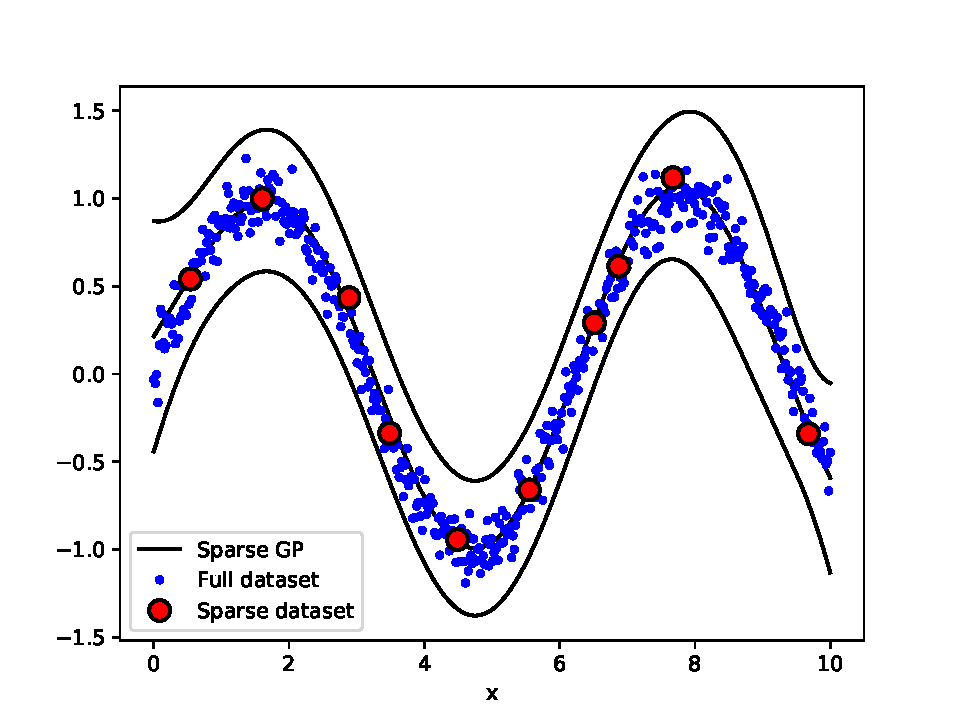
\includegraphics[scale=0.7]{1D_example_results.pdf}
	\caption{Example output of `1D\_example' Python script.}
	\label{fig:example_results}
\end{figure}

Note that a more thorough approach to this problem would be to recursively add additional training points and update the GP hyperparameters. In  \cite{Titsias2009}\cite{Titsias2009a} it is shown that the lower bound, $L_{lb}$, must increase every time an additional training point is included. This is convenient, as it allows the user to analyse convergence - new training points and hyperparameter updates can be run until $L_{lb}$ is judged to have converged. For now though, for the sake of simplicity, our example code simply tries to identify a fixed number of training points (and optimum hyperparameters) for the Sparse GP implementation. \\

%%%%%%%%%%%%%%%%%%%%%%%%%%%%%%%%%%%%%%%%%%%%%%%%%%%%%%%%%%%%%%%%%%%%%%%%%%
\section{Detailed Methodology}\label{sec:details}
Defining a prior $p(\f,\f_m)$ and likelihood $p(\y|\f,\f_m)$ gives us the posterior

\begin{equation}
	p(\f,\f_m|\y) = \frac{p(\y|\f,\f_m)p(\f,\f_m)}{p(\y)}
\end{equation}
We decide that the optimum choice of $\f_m$ would lead to

\begin{equation}
	p(\y|\f_m) = p(\y|\f,\f_m)
\end{equation}
In other words, if we knew the optimum $\f_m$ then, regarding the probability of witnessing $\y$, $\f$ doesn't add any additional information\footnote{Sometimes in the literature optimality is defined as $p(\f,\f_m|\y)=p(\f|\f_m)$. In fact, expanding both sides using Bayes' theorem you can show that $p(\f,\f_m|\y)=p(\f|\f_m) \implies p(\y|\f_m) = p(\y|\f,\f_m)$ so it doesn't make any difference. I prefer stating that $p(\y|\f_m) = p(\y|\f,\f_m)$ is the optimal condition as it seems a bit more intuitive.}. It turns out that the optimum $\f_m$ will factorise the posterior, so that we can write $p(\f,\f_m|\y)=p(\f|\y)p(\f_m|\y)$. Proof:

\begin{equation}
	p(\f,\f_m|\y) = \frac{p(\y|\f_m)p(\f,\f_m)}{p(\y)} 
\end{equation}

\begin{equation}
	= \frac{p(\y|\f_m)p(\f_m|\f)p(\f)}{p(\y)} \times \frac{p(\f_m)}{p(\f_m)}
\end{equation}

\begin{equation}
	= \frac{p(\f_m|\f)p(\f)}{p(\f_m)} \frac{p(\y|\f_m)p(\f_m)}{p(\y)}
\end{equation}

\begin{equation}
	=p(\f|\f_m)p(\f_m|\y)
\end{equation}
So in the optimal case we can factorise the posterior pdf as

\begin{equation}
	p(\f,\f_m|\y) = p(\f_m|\y)p(\f|\f_m)
\end{equation}
For this reason, we choose a variational distribution \emph{which can be factorised in the same way} by defining

\begin{equation}
	q(\f,\f_m) = \phi(\f_m) p(\f|\f_m)
\end{equation}
and we try to minimise the KL divergence between $q(\f,\f_m)$ and the posterior $p(\f,\f_m|\y)$. This is based on the hypothesis that, if we find inputs $\X_m$ that make $q(\f,\f_m) = \phi(\f_m) p(\f|\f_m)$ and $p(\f,\f_m|\y)$ exactly the same, then it must be possible to factorise the posterior distribution into $p(\f_m|\y)p(\f|\f_m)$, thus implying that our choice of $\X_m$ is optimal. Noting that minimising

\begin{equation}
	\text{KL}(q(\f,\f_m) || p(\f,\f_m|\y))
\end{equation}
is equivalent to maximising

\begin{equation}
	L = \int \int q(\f,\f_m) \log \left[ \frac{p(\f,\f_m,\y)}{q(\f,\f_m)} \right] d\f d\f_m
\end{equation}
then, by enforcing the factorisation property of the variational distribution ($q(\f,\f_m) = \phi(\f_m) p(\f|\f_m)$) and writing $p(\f,\f_m,\y) = p(\y|\f)p(\f|\f_m)p(\f_m))$ we have

\begin{equation}
	L = \int \int p(\f|\f_m) \phi(\f_m) \log \left\{ \frac{p(\y|\f)p(\f_m)}{\phi(\f_m)} \right\} d\f d\f_m
\end{equation}

\begin{equation}
	= \int \phi(\f_m) \underbrace{\left[  \int p(\f|\f_m)\log p(\y|\f) d\f \right]}_{\log G(\f_m,\y)}  + \log \left( \frac{p(\f_m)}{\phi(\f_m)} \right) d\f_m
\end{equation}
To evaluate $\log G = \int p(\f|\f_m)\log p(\y|\f) d\f $, we first need to find an expression for $p(\f|\f_m)$. Noting that

\begin{equation}
	p(\f,\f_m) = \mathcal{N}\left(
	\left(
	\begin{array}{c}
		\f \\
		\f_m \\
	\end{array}
	\right);
	\boldsymbol{0}, \left[
	\begin{array}{cc}
		\boldsymbol{K}_{nn} & \boldsymbol{K}_{nm}\\
		\boldsymbol{K}_{mn} & \boldsymbol{K}_{mm} \\
	\end{array}
	\right]
	\right)
\end{equation}
where $\boldsymbol{K}_{nn}(i,j) = k(\x_i,\x_j)$, $\boldsymbol{K}_{nm}(i,j) = k(\x_i,\x_{m,j})$ and $\boldsymbol{K}_{mm}(i,j) = k(\x_{m,i},\x_{m,j})$. Using standard properties of Gaussian distributions we can then show that

\begin{equation}
	p(\f|\f_m) = \mathcal{N}(\f; \boldsymbol{0}, \E[\f|\f_m],\Cov[\f|\f_m])
\end{equation}
where

\begin{equation}
	\E[\f|\f_m] = \boldsymbol{K}_{nm} \boldsymbol{K}_{mm}^{-1} \f_m
\end{equation}
and

\begin{equation}
	\Cov[\f|\f_m] = \boldsymbol{K}_{nn} - \boldsymbol{K}_{nm}\boldsymbol{K}_{mm}^{-1}\boldsymbol{K}_{mn}
\end{equation}
We can now try to evaluate $\log G$. To simplify notation, we first define $\bmu = \E[\f|\f_m]$ and $\bSigma = \Cov[\f|\f_m]$ such that the aim is to evaluate

\begin{equation}
	\log G = \int \mathcal{N}(\f;\bmu,\bSigma) \log p(\y|\f) d\f
\end{equation}
where

\begin{equation}
	\log p(\y|\f) = -\frac{N}{2} \log (2\pi\sigma^2) - \frac{1}{2\sigma^2} \sum_{i=1}^N (y_i - f_i)^2
\end{equation}
therefore 

\begin{equation}
	\log G = \int \mathcal{N}(\f;\bmu,\bSigma) \left[  
		-\frac{N}{2}\log(2\pi\sigma^2) -\frac{1}{2\sigma^2} \sum_{i=1}^N (y_i-f_i)^2
	\right] d\f
\end{equation}

\begin{equation}
	= -\frac{N}{2} \log(2\pi\sigma^2) - \frac{1}{2\sigma^2} \sum_{i=1}^N \underbrace{\left[
		\int \mathcal{N}(f_i;\mu_i,\Sigma_{ii}) (y_i-f_i)^2 df_i
	\right]}_{I}
\end{equation}
Noting that we can write

\begin{equation}
	(y_i-f_i)^2 = \left( y_i^2 - 2f_i y_i + (f_i-\mu_i^2) \right) + 2f_i\mu_i - \mu_i^2
\end{equation}
then the intergral $I$ becomes

\begin{equation}
	y_i^2 - 2\mu_i y_i + \mu_i^2 + \Sigma_{ii} = (y_i-\mu_i)^2 + \Sigma_{ii}
\end{equation}
therefore

\begin{equation}
	\log G = -\frac{N}{2}\log(2\pi\sigma^2) - \frac{1}{2\sigma^2} \sum_{i=1}^N \left[ (y_i-\mu_i)^2 + \Sigma_{ii} \right]
\end{equation}

\begin{equation}
	= \log(\mathcal{N}(\y;\bmu,\boldsymbol{I}_N\sigma^2)) -\frac{1}{2\sigma^2}\Tr(\bSigma)
\end{equation}
This is a good point to summarise what we've done so far! We want to find the inputs, $\X_m$, that maximise 

\begin{equation}
	L = \int \phi(\f_m) \left[
		\log G(\f_m,\y) + \log \left(  \frac{p(\f_m)}{\phi(\f_m)} \right) d\f_m
	\right]
\end{equation}
where

\begin{equation}
	\log G = \log \left(  \mathcal{N}(\y;\E[\f|\f_m],\boldsymbol{I}_N\sigma^2) \right) -\frac{1}{2\sigma^2}\Tr\left( \Cov[\f|\f_m] \right)
\end{equation}

\begin{equation}
	\E[\f|\f_m] = \boldsymbol{K}_{nm} \boldsymbol{K}_{mm}^{-1} \f_m
\end{equation}
and

\begin{equation}
	\Cov[\f|\f_m] = \boldsymbol{K}_{nn} - \boldsymbol{K}_{nm}\boldsymbol{K}_{mm}^{-1}\boldsymbol{K}_{mn}
\end{equation}
Noting that we can write 

\begin{equation}
	L = \int \phi(\f_m) \left[
		\log \left( G(\f_m,\y)  \frac{p(\f_m)}{\phi(\f_m)} \right)
	\right] d\f_m
\end{equation}
then, using Jensen's inequality, we can now calculate a lower bound on $L$:

\begin{equation}
	L \geq L_{lb} = \log \left[  \int \phi(\f_m) \frac{G(\f_m,\y) p(\f_m)}{\phi(\f_m)}  d\f_m \right]
\end{equation}

\begin{equation}
	= \log \int G(\f_m,\y)p(\f_m) d\f_m
\end{equation}
Note that, to maximise $L_{lb}$, we don't actually have to find the variational distribution $\phi(\f_m)$ (a nice trick!). To evaluate the lower bound:

\begin{equation}
	L_{lb} = \log \underbrace{\left[ \int \mathcal{N}(\y;\E[\f|\f_m],\boldsymbol{I}_N \sigma^2) p(\f_m) d\f_m \right]}_{I_2} -\frac{1}{2\sigma^2} \Tr\left( \Cov[\f|\f_m] \right)
	\label{eq:kalman_integral}
\end{equation}
The integral $I_2$ can be evaluated using standard expressions for Gaussian distributions (see Appendix \ref{appendix_integral}) such that, finally, we have our objective function:

\begin{equation}
	L_{lb} = \log \left[ \mathcal{N}(\y; \boldsymbol{0}, \boldsymbol{I}_n\sigma^2 + \boldsymbol{K}_{nm}\boldsymbol{K}_{mm}^{-1}\boldsymbol{K}_{mn}) \right] -\frac{1}{2\sigma^2} \Tr\left(  \Cov[\f|\f_m] \right)
\end{equation}
where $\Cov[\f|\f_m] = \boldsymbol{K}_{nn} - \boldsymbol{K}_{nm}\boldsymbol{K}_{mm}^{-1}\boldsymbol{K}_{mn}$. 


%%%%%%%%%%%%%%%%%%%%%%%%%%%%%%%%%%%%%%%%%%%%%%%%%%%%%%%%%%%%%%%%%%%%%%%%%%
\section{Some Interesting References}\label{sec:refs}
\cite{Lazaro-Gredilla2011} produced a Variational Sparse GP that could also treat heterscedastic problems. \cite{Chai2012} specifically considered classification but, in the process, looked into how a Variational Sparse GP could be applied when there are non-conjugate likelihoods. \cite{Damianou2012} introduced `Deep Gaussian Processes' (A deep belief network based on GP mappings), where variational GPs was central to the approach. They showed that Deep GPs are applicable to large data sets (like other deep methods but also small data sets (unlike other deep methods). This was illustrated on a case study with more dimensions than data. \cite{Hensman2013} produced a variant of Variational Sparse GPs that is suitable for stockastic variational inference. This was applied to datasets with around 700,000 points. \cite{Hensman2014} looked at Deep GPs again and proposed a `nested' approach to variational inference that makes them more suitable for parallel computer architectures. Notes the danger of overfitting when using deep methods. \cite{Gal2014} proposed a Variational Sparse GP that is suitable for a Map-Reduce setting and applied to datasets with around 2 million data points (implemented on open-source MapReduce software in Python). \\

It is worth noting that, while these datasets are quite large, \cite{Deisenroth2015} presented the `robust Bayesian Committee Machine' (extension of a product-of-experts model) that was applicable to data sets of the order $10^7$. They also have some interesting criticisms of Sparse GPs, particularly with regard to the number of parameters that need to be trained. \\

Finally, Sparse GP code is available for free through the University of Sheffield's Python module GPy. Other interesting variants of GPs for large data sets can also be found in \cite{Wilson2015}\cite{Wilson2015a}. \\

%%%%%%%%%%%%%%%%%%%%%%%%%%%%%%%%%%%%%%%%%%%%%%%%%%%%%%%%%%%%%%%%%%%%%%%%%%
\newpage
\appendix
\section{Evaluating equation (\ref{eq:kalman_integral})}\label{appendix_integral}
Generally speaking, for the situation where

\begin{equation}
	p(\x_a) = \mathcal{N}(\x_a; \boldsymbol{\mu}, \boldsymbol{A}^{-1}), \qquad p(\x_b | \x_a) = \mathcal{N}(\x_b; \boldsymbol{H}\x_a + \boldsymbol{b}, \boldsymbol{L}^{-1})
\end{equation}
it can be shown that

\begin{equation}
	p(\x_b) = \int p(\x_b | \x_a) p(\x_a) d\x_a = \mathcal{N}(\x_b; \boldsymbol{H}\boldsymbol{\mu} + \boldsymbol{b}, \boldsymbol{L}^{-1}\boldsymbol{HA}^{-1}\boldsymbol{H}^T)
\end{equation}
This is proved, for example, in Bishop's book \cite{bishop2006pattern} and also forms part of the derivation of the well-known Kalman filter equations. Applying this generalised result to the integral in equation (\ref{eq:kalman_integral}), we find the following:

\begin{equation}
	\int \mathcal{N} \left( \y; \boldsymbol{K}_{nm} \boldsymbol{K}_{mm}^{-1} \boldsymbol{f}_m, \boldsymbol{I}_n \sigma^2 \right)
	\mathcal{N}\left( \boldsymbol{f}_m; \boldsymbol{0}, \boldsymbol{K}_{mm} \right) d \boldsymbol{f}_m
\end{equation}

\begin{equation}
	= \mathcal{N} \left( \y; \boldsymbol{0}, \boldsymbol{I}_n \sigma^2 + \boldsymbol{K}_{nm}\boldsymbol{K}_{mm}^{-1}\boldsymbol{K}_{mm} \boldsymbol{K}_{mm}^{-T} \boldsymbol{K}_{mn} \right)
\end{equation}

\begin{equation}
	= \mathcal{N} \left( \y; \boldsymbol{0}, \boldsymbol{I}_n \sigma^2 + \boldsymbol{K}_{nm} \boldsymbol{K}_{mm}^{-1} \boldsymbol{K}_{mn} \right)
\end{equation}









\bibliography{bibliography}
\bibliographystyle{unsrt}

\end{document} 
